
\section{Use Cases}

The main idea of this project is to convert a markdown file into a pdf/html/css file. To do this, the computer must first convert the markdown file into C++ data. This comes in line with the first Use Case where the user requested a conversion of some sort and to fulfill that, the system must first take the file and then properly convert to C++ data. From there based on the user's request, the C++ data can be used to generate a pdf (such as with Use Case 2) or even an html or css output. \\
The main error scenerios could occur between any of the conversion points. For instance, between markdown to C++ data, the C++ would need to accurately represent the markdown otherwise when it would go on to be converted to a pdf/html/css, it would not match the markdown. Other error scenerios could occur with reading and actually converting the markdown without any errors. \\
\textbf{Use Case Name:} Markdown to C++ data  
\\
\textbf{Goal:} Converts a given markdown file to C++ data
\\
\textbf{Actor:} Computer converting between markdown and pdf/html/css 
\\
\textbf{Preconditions:} 
\begin{itemize}
\item A user has requested that the program convert their markdown file into either pdf/html/css 
\item In order to produce the correct output, the computer needs to convert the markdown into C++ data 
\item Program is able to open and read the markdown file
\end{itemize}
\textbf{Postconditions:} 
\begin{itemize}
\item Markdown file is available as C++ data for the program to further use in converting to desired file type  
\item The C++ data accurately represents the markdown file
\end{itemize}
\textbf{Flow of Events:} 
\begin{itemize}
\item System reads in the markdown file that the user has provided 
\item The markdown file is converted into C++ data 
\item The system now has the C++ data 
\end{itemize}
\textbf{Quality Requirements:} 
\begin{itemize}
\item The user will be notified of any issues in the conversion between C++ data and either to the PDF and the HTML. If there are errors in the conversion the user will be notified and re-prompted if they could remedy the situation such as with a file misread.
\item The system will process the C++ data in timely manner, depending on the input size. If the process ends up taking too long given a large input, the user has the choice to exit. 
\end{itemize}
\textbf{Use Case Name:} PDF Output  
\\
\textbf{Goal:} Allows to convert from markdown to pdf data
\\
\textbf{Actor:} Person needing pdf version of their markdown file
\\
\textbf{Preconditions:} 
\begin{itemize}
\item Markdown file has been created and written to by user 
\item The system has already converted the markdown file into C++ data
\item The C++ data is available and ready for access 
\end{itemize}
\textbf{Postconditions:} 
\begin{itemize}
\item Markdown file is available as a pdf file 
\item User is able to view and access the pdf version
\item The pdf version is accurate to the markdown file that was provided 
\end{itemize}
\textbf{Flow of Events:} 
\begin{itemize} 
\item User has requested a pdf file
\item The system then takes the C++ data and turns it into pdf data 
\item The pdf data is then presented to the user 
\end{itemize}
\textbf{Quality Requirements:} 
\begin{itemize}
\item The user will be notified of any issues in the conversion. Then with any errors such as file-misread, the user will be notified, and depending on issue reprompted. 
\item The system will process the pdf data in timely manner, depending on the input size. With a large input the time may be longer and so the user would have the option to halt the process. 
\item The pdf version will accurately represent the markdown that the user had originally provided. With any differences caused by errors, the user would be notified and so is made aware.
%
\end{itemize} 
\textbf{Use Case Name:} .html/.css Output  
\\
\textbf{Goal:} Allows to convert from markdown to .html/.css data
\\
\textbf{Actor:} Person needing .html/.css version of their markdown file
\\
\textbf{Preconditions:} 
\begin{itemize}
\item Markdown file has been created and written to by user 
\item The system has already converted the markdown file into C++ data
\item The C++ data is available and ready for access 
\end{itemize}
\textbf{Postconditions:} 
\begin{itemize}
\item Markdown file is available as .html/.css file 
\item User is able to view and access the .html/.css version
\item The .html/.css version is accurate to the markdown file that was provided 
\end{itemize}
\textbf{Flow of Events:} 
\begin{itemize} 
\item User has requested .html/.css file
\item The system then takes the C++ data and turns it into .html/.css data 
\item The .html/.css data is then presented to the user 
\end{itemize}
\textbf{Quality Requirements:} 
\begin{itemize}
\item The user will be notified of any issues in the conversion. Again with any issues that could be fixed with user input such file read in, the user will be reprompted. 
\item The system will process the .html/.css data in timely manner, depending on the input size. If time ends up taking longer than user wished due to lengthly input, the user has the option to stop the conversion.  
\item The .html/.css version will accurately represent the markdown that the user had originally provided. With any known errors that lead to differences, the user will be notified. 
%
\end{itemize} 


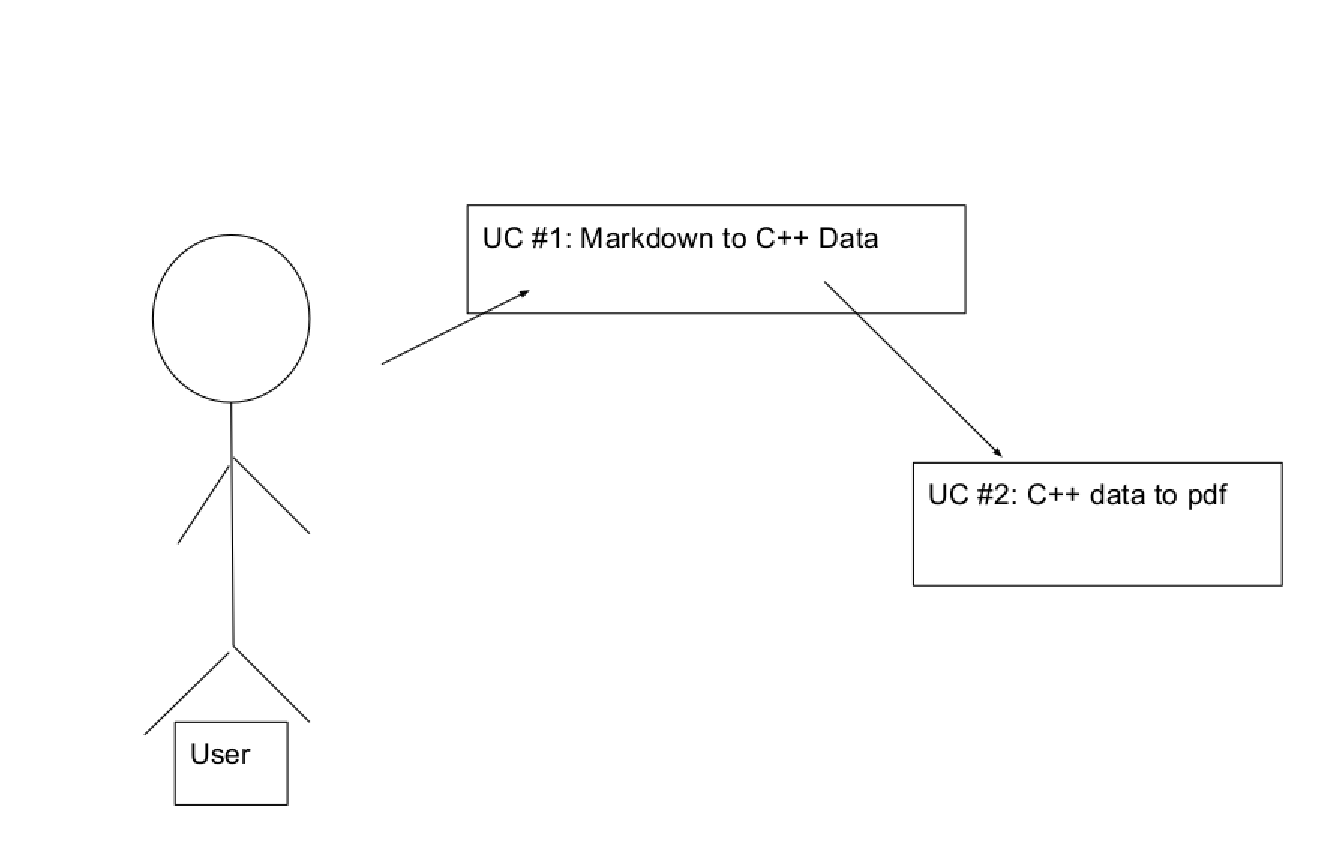
\includegraphics[width=300pt]{images/useCase.eps}
